\subsection{Query Skeleton Creation}
\label{sec:skeleton}

In this step, our technique scans the provided input and output examples, guesses
what a target SQL query might look like, and infers a set of query skeletons
that capture the basic query structures.

A query skeleton is an incomplete SQL query, which
captures three basic query structures that could
often be decided after a simple scan over the examples:
tables used in a result SQL
query, table columns used to join input tables, and table
columns for projecting the query results. Other parts in a SQL query such as conditions
(including selection and having conditions), and aggregations
are left as unkown, and will be determinated in the next step (Section~\ref{sec:completion}).



%\begin{itemize}

%\item
\vspace{1mm}
\noindent \textit{\textbf{Step 1: Determining the Table Set.}} 
In practice, end-users are unwilling to provide more than enough
inputs. Therefore, every input table specified in the example
is expected to be used to construct a desirable SQL query.
Based on this observation, we assume that every input table
should be used as least once in the query. By default, the
table set $T$ used in the result SQL query contains all given input tables.
However, it is possible that a single table will be used for multiple times.
Our technique does not forbid this case, rather, we adopt a single heuristic
to estimate the used table set: if the same column from an input table appears more than once in the
example output, we add the input table the same number of times to the used table set.

%we view it as a strong indicator that this table will be joined multiple times and add it to our table
%set $T$ using an alias.


%\item
\vspace{1mm}
\noindent\textit{\textbf{Step 2: Determining Joining Columns. }} Given two arbitrary tables, there exist many
ways to join them. Enumerating all possible joining conditions may introduce a huge number of joining
conditions and would quickly become intractable. We observe that, in practice, two tables are often joined via the following
three cases: (1) tables are joined on their primary keys with the same (or compatible) data types, such
as joining a \textit{student} table with an \textit{enrolled} table with the \textit{student\_id} column. It does not
make any sense to join two tables on a Integer column and a String column; (2) tables are joined
using columns with the same name, such as joining a \textit{student} table with a \textit{enrolled} table on the
\textit{student\_name} column; and (3) two columns that have the data type, and have a large portion of
overlapped values in their corresponding input tables can be used as a joining condition. It is straightforward to check the first 
two cases to identify possible joining columns. For the third case, our technique scans the given input tables to check ``value similarity''
between two arbitrary columns, and selects columns whose ``value similarity'' is above a fixed threshold as joining columns.
\todo{need to implement above.}
\todo{mention how many skeletons will be created}

%\item
\vspace{1mm}
\noindent \textit{\textbf{Step 3: Determining Output Columns.}} To identify output table columns on
which the querying result would be projected, our technique checks whether each output
table column name appears in any input tables. If so, we used the matched column
from the input table as the output column. Otherwise, the output column
must be produced by using aggregation. Our technique keeps track of those aggregation columns
and search for proper aggregates in the next phase (Section~\ref{sec:agg_search}). 
\todo{check the values in the output column}

%After determining the table set and joining columns,
%the next step is to identify potential column names on which the result would be projected. If a
%column in the output table  does not appear in any input table's column list, this output column must
%be produced by aggregation. Our algorithm keeps track of these columns and appends a \CodeIn{group by} ... \CodeIn{having} ...
%clause to the query skeleton.

%\end{itemize}
\vspace{1mm}

In summary, this step infers three parts as a query skeleton: tables used in constructing a SQL query, joining conditions
to connect the input tables, and a list of columns to project the output results.

%It is worth noting that the results obtained from the above steps are not \textit{safe} in
%terms that they may miss some valid SQL queries. 

%We made the above assumption for the sake of tractability,
%since in theory, the bound of table number in a SQL query is $O(n_t!)$, where $n_t$ is the number of given tables;
%while the bound of possible number of join is $O(c_t^2)$ and the bound of the number of conditions is $O(n_t!n_tc_t^2)<O(n_t^3c_t^2)$.

%\subsubsection{Inferring Output Table Schema}

%Lacks schema

\subsubsection{Example}

For our motivating example, from the output table (Figure~\ref{tbl:output}), our technique identifies that
column {\CodeIn{Student\_name}} comes from table \CodeIn{student} and
column {\CodeIn{Max\_Score}} is a new one which must be created by using aggregation.
% which indicates aggregation and group by.

%while the bound of possible number of join is $O(c_t^2)$ and the bound of the number of conditions is $O(n_t!n_tc_t^2)<O(n_t^3c_t^2)$.

\begin{figure}[t]
	\centering
%\begin{CodeOut}
%\begin{alltt}
%\textbf{select student.Student\_name, $\color{blue}{<Aggregate>}$ 
%from student, enrolled
%where student.Student\_key = course.Student\_key
%      and \color{red}{<Conditions>}
%group by student.Student\_key
%having \color{red}{<Conditions>}}
%\end{alltt}
%\end{CodeOut}
%\vspace{-5mm}
		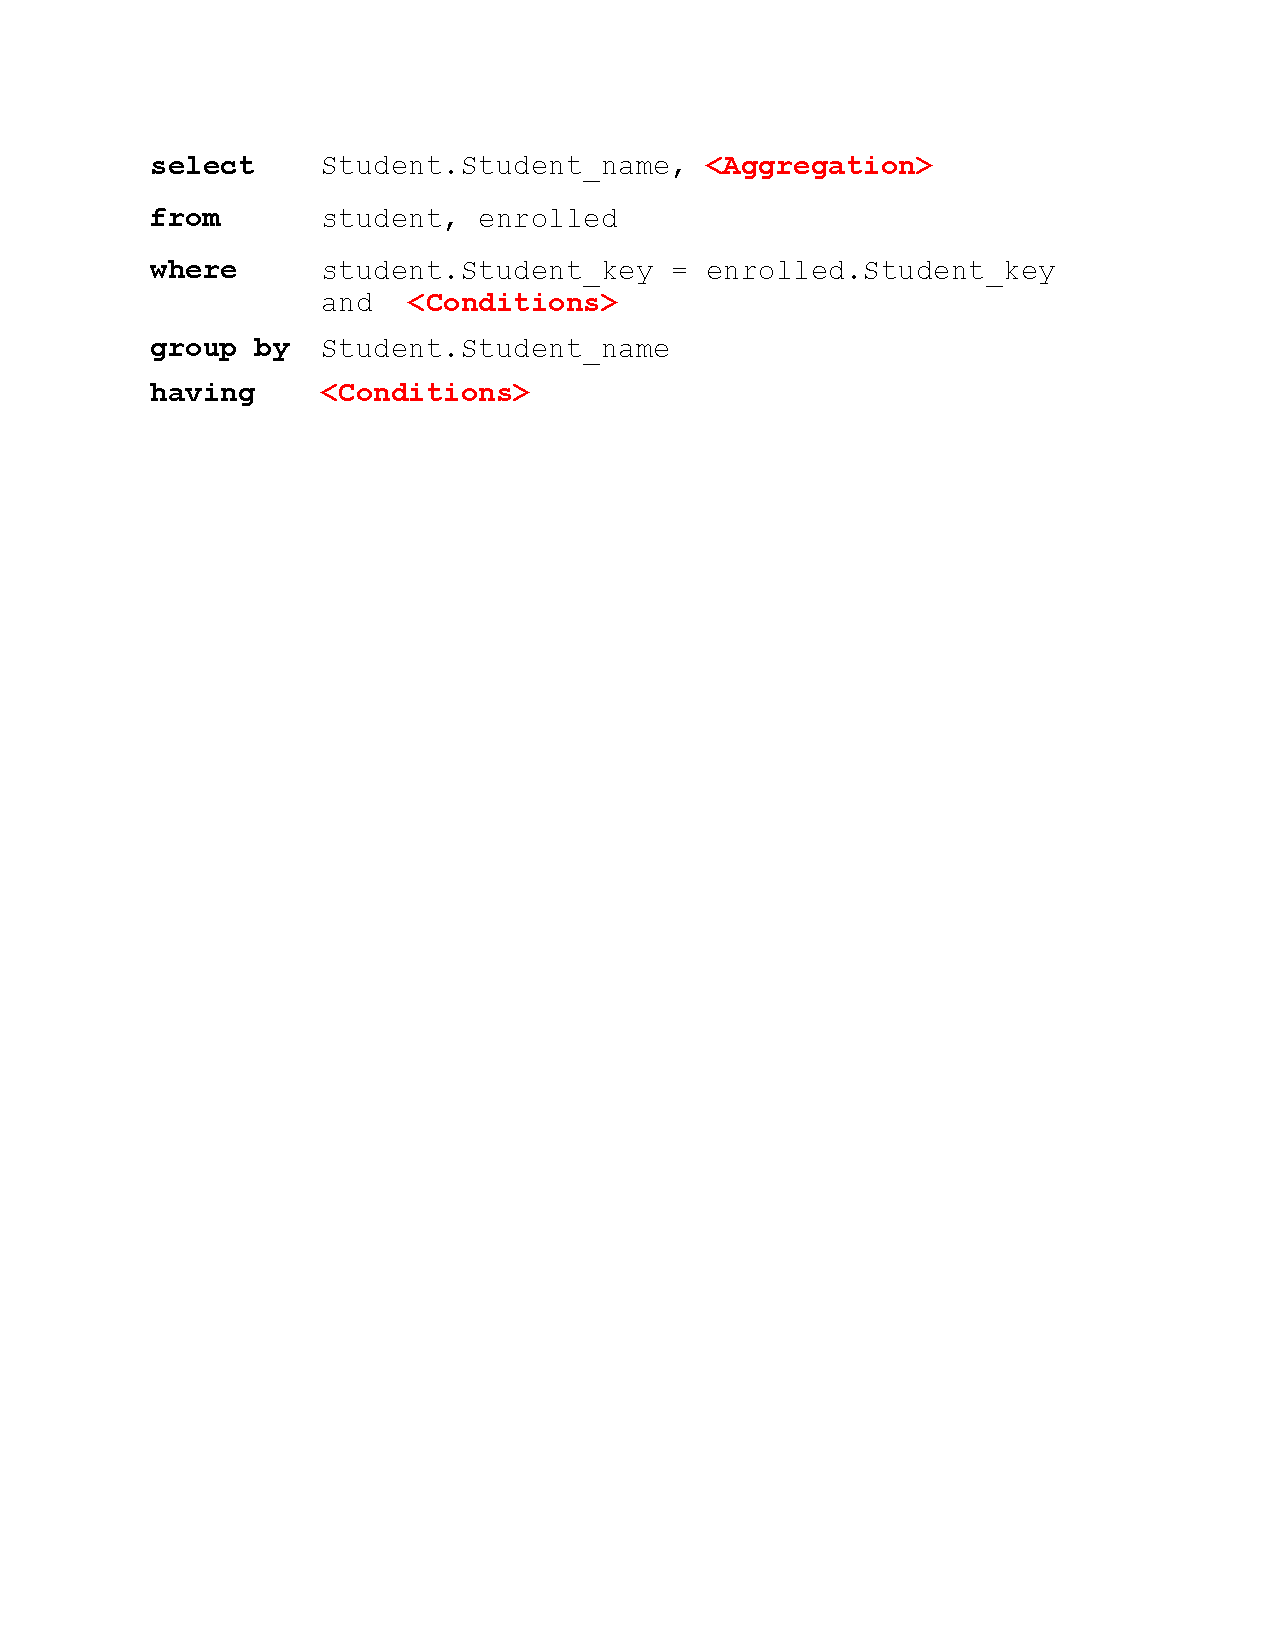
\includegraphics[width=0.45\textwidth]{sql_skeleton.pdf}
	\caption{The SQL skeleton created for the motivating example
in Section~\ref{sec:example}.}
	\label{fig:skeleton}
\end{figure}

The created query skeleton  is shown in Figure \ref{fig:skeleton}.
As we can see from Figure \ref{fig:skeleton},  there are three unknown structures represented
by $<$Aggregation$>$ or $<$Conditions$>$ in red color, which will be filled in the next phase.
